% !TEX encoding = UTF-8
% !TEX TS-program = pdflatex
% !TEX root = ../tesi.tex
% !TEX spellcheck = it-IT

%**************************************************************
\chapter{Progettazione e codifica}
\label{cap:progettazione-codifica}
%**************************************************************

\intro{Breve introduzione al capitolo}\\

%**************************************************************

\section{Angular MVC}
AngularJS è stato il framework maggiormente utilizzato in questo stage e mi ha consentito di implementare l'intero progetto agilmente.\\
Alla base del framework, è collocato il design pattern \gls{mvc}, leggermente modificato per adattarsi alle funzionalità di AngularJS. Il design pattern che ne risulta è qualcosa di più flessibile del classico \gls{mvc}, consentendo agli sviluppatori una maggior libertà di utilizzo.\\
Ovviamente ci sono delle direttive e delle best practice consigliate, soprattutto se si intende creare un \gls{frontend} davvero \gls{rest}-ful.

\subsection{Two-way Data Binding}
Una funzionalità importante che AngularJS espone è il cosiddetto \emph{Two Way Data Binding}. Si parla di \emph{legame doppio tra dati} quando una variabile del modello è legata ad un elemento che può cambiare ed al contempo mostrare il contenuto della variabile stessa. In una vista di AngularJS, ogniqualvolta un elemento che applica il \emph{Two Way Data Binding} viene modificato, il corrispondente campo nel modello viene notificato e aggiornato correttamente.\\
In AngularJS, si usa la direttiva \textbf{ng-model} per legare una variabile del modello ad un elemento \gls{html} che può sia mostrare il suo valore, che modificarlo.

\begin{figure}[H] 
    \centering 
    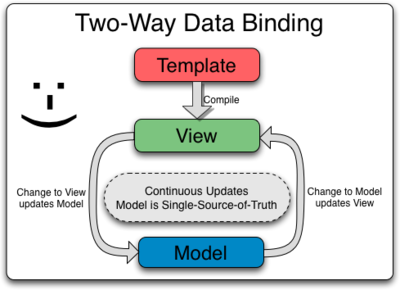
\includegraphics[width=0.8\columnwidth]{two_way_data_binding} 
    \caption{Doppio legame tra vista e modello di AngularJS}
\end{figure}




%**************************************************************

\section{Tecnologie e strumenti}
\label{sec:tecnologie-strumenti}

Di seguito viene data una panoramica delle tecnologie e strumenti utilizzati.

\subsection*{Tecnologia 1}
Descrizione Tecnologia 1.

\subsection*{Tecnologia 2}
Descrizione Tecnologia 2

%**************************************************************
\section{Ciclo di vita del software}
\label{sec:ciclo-vita-software}

%**************************************************************
\section{Progettazione}
\label{sec:progettazione}

\subsubsection{Namespace 1} %**************************
Descrizione namespace 1.

\begin{namespacedesc}
    \classdesc{Classe 1}{Descrizione classe 1}
    \classdesc{Classe 2}{Descrizione classe 2}
\end{namespacedesc}


%**************************************************************
\section{Design Pattern utilizzati}

%**************************************************************
\section{Codifica}
